\documentclass[11pt, oneside]{article}   	% use "amsart" instead of "article" for AMSLaTeX format
\usepackage{geometry}                		% See geometry.pdf to learn the layout options. There are lots.
\geometry{letterpaper}                   		% ... or a4paper or a5paper or ... 
%\geometry{landscape}                		% Activate for rotated page geometry
%\usepackage[parfill]{parskip}    		% Activate to begin paragraphs with an empty line rather than an indent
\usepackage{graphicx}				% Use pdf, png, jpg, or eps§ with pdflatex; use eps in DVI mode
								% TeX will automatically convert eps --> pdf in pdflatex		
\usepackage{amssymb}

%SetFonts

%SetFonts


\title{Brief Article}
\author{The Author}
%\date{}							% Activate to display a given date or no date

\begin{document}
\begin{flushright}
Donovan Guelde\\
CSCI 5454 PS4\\
Collaborators: NONE\\
\end{flushright}
1.  \underline{Results from Game 1:}\\\\
econ1-135-3-dhcp:ps4 donovanjamesguelde\$ python q1algo.py\\
Choose game\\
1: player vs AI\\
2: AI vs AI\\
Enter 1 or 2:1\\
enter bounds for matrix values, separated by a comma (ex: 1,5): 1,20\\
number of rounds: 20\\
\\
Results of game\_value():\\
Column Player Weights:\\
\indent 4.28134220e-01   6.88595617e-08   2.64080008e-10   5.71865711e-01   1.41177675e-11\\
Row Player Weights:\\
\indent 3.10921036e-01   1.64528454e-06   6.68154265e-01   1.21027747e-04   2.08020256e-02\\
Game Value: 12.3371644896\\
Expected Score: 246.743289791\\
\\
Payoff Matrix:\\

\begin{tabular}{ c c c c c}
 19 & 20 &  1 &  9 & 10\\
   8 &  6 & 11 & 18  & 5\\
   9 &  2 & 10 & 14 &  4\\
   9  & 6 &  7 & 16 & 20\\
  17 & 14 &  1 & 11 &  4\\
\end{tabular}
\\
\\
column played: 3   Row Played: 3 Payoff: 16.0\\
column played: 3   Row Played: 3 Payoff: 16.0\\
column played: 3   Row Played: 0 Payoff: 9.0\\
column played: 3   Row Played: 0 Payoff: 9.0\\
column played: 3   Row Played: 2 Payoff: 14.0\\
column played: 3   Row Played: 1 Payoff: 18.0\\
column played: 3   Row Played: 4 Payoff: 11.0\\
column played: 3   Row Played: 4 Payoff: 11.0\\
column played: 3   Row Played: 4 Payoff: 11.0\\
column played: 0   Row Played: 4 Payoff: 17.0\\
column played: 0   Row Played: 4 Payoff: 17.0\\
column played: 0   Row Played: 1 Payoff: 8.0\\
column played: 0   Row Played: 1 Payoff: 8.0\\
column played: 3   Row Played: 4 Payoff: 11.0\\
column played: 3   Row Played: 3 Payoff: 16.0\\
column played: 3   Row Played: 3 Payoff: 16.0\\
column played: 3   Row Played: 0 Payoff: 9.0\\
column played: 3   Row Played: 2 Payoff: 14.0\\
column played: 3   Row Played: 4 Payoff: 11.0\\
column played: 0   Row Played: 2 Payoff: 9.0\\
Column Player Score: 251.0\\
Column Player Expected Score: 246.743289791\\
\\ 
\\
\\
\indent \underline{Results from Game 2:}\\\\
econ1-135-3-dhcp:ps4 donovanjamesguelde\$ python q1algo.py
Choose game\\
1: player vs AI\\
2: AI vs AI\\
Enter 1 or 2:1\\
enter bounds for matrix values, separated by a comma (ex: 1,5): -10,10\\
number of rounds: 20\\
\\
Results of game\_value():\\
Column Player Weights:\\
\indent 2.11954718e-01   2.14740265e-06   1.01895578e-01   6.86147557e-01   4.91353672e-12\\
Row Player Weights:\\
\indent 3.23439627e-01   6.30161952e-02   3.30781076e-11   6.37058125e-02   5.49838365e-01\\
Game Value: 0.646927680315\\
Expected Score: 12.9385536063 \\
\\
Payoff Matrix:\\
\begin{tabular}{ c c c c c}
 -3  &-4  & 9 & -1  & 0\\
 -10 & -8 & -2 &  4  & 2\\
   0 &-10  & 3 &  6 & -8\\
   5  & 1  & 2  & 0  & 7\\
   3  & 0 & -1  & 1 & -9\\
\end{tabular}
\\
\\
column played: 2   Row Played: 4 Payoff: -1.0\\
column played: 2   Row Played: 2 Payoff: 3.0\\
column played: 2   Row Played: 4 Payoff: -1.0\\
column played: 2   Row Played: 1 Payoff: -2.0\\
column played: 2   Row Played: 4 Payoff: -1.0\\
column played: 0   Row Played: 3 Payoff: 5.0\\
column played: 0   Row Played: 3 Payoff: 5.0\\
column played: 0   Row Played: 1 Payoff: -10.0\\
column played: 3   Row Played: 4 Payoff: 1.0\\
column played: 3   Row Played: 2 Payoff: 6.0\\
column played: 3   Row Played: 0 Payoff: -1.0\\
column played: 3   Row Played: 2 Payoff: 6.0\\
column played: 3   Row Played: 0 Payoff: -1.0\\
column played: 2   Row Played: 1 Payoff: -2.0\\
column played: 2   Row Played: 3 Payoff: 2.0\\
column played: 2   Row Played: 0 Payoff: 9.0\\
column played: 2   Row Played: 3 Payoff: 2.0\\
column played: 2   Row Played: 4 Payoff: -1.0\\
column played: 2   Row Played: 4 Payoff: -1.0\\
column played: 2   Row Played: 0 Payoff: 9.0\\
Column Player Score: 27.0\\
Column Player Expected Score: 12.9385536063\\
\\
\\
\indent \underline{Results from Game 3:}\\\\
econ1-135-3-dhcp:ps4 donovanjamesguelde\$ python q1algo.py\\
Choose game\\
1: player vs AI\\
2: AI vs AI\\
Enter 1 or 2:1\\
enter bounds for matrix values, separated by a comma (ex: 1,5): -20,20\\
number of rounds: 20\\
\\
Results of game\_value():\\
Column Player Weights:\\
\indent 4.31366390e-08   1.61089163e-01   3.73812918e-01   2.09789091e-01   2.55308784e-01\\
Row Player Weights:\\
\indent2.10995340e-01   3.81329776e-01   2.06835582e-01   2.00815047e-01   2.42553041e-05\\
Game Value: 0.528087144092\\
Expected Score: 10.5617428818 \\
\\
Payoff Matrix:\\
\begin{tabular}{c c c c c}
-16 & -16 & 15 & -5 &  9\\
 -11 & 13 &  1 & -4 & -7\\
  20 &-13 & 10  &14& -19\\
 -18 &  4& -12 &  0 & 10\\
 1 & 16 & 20 &-11  & 7\\
\end{tabular}
\\
\\
column played: 2   Row Played: 3 Payoff: -12.0\\
column played: 2   Row Played: 4 Payoff: 20.0\\
column played: 2   Row Played: 3 Payoff: -12.0\\
column played: 2   Row Played: 4 Payoff: 20.0\\
column played: 2   Row Played: 0 Payoff: 15.0\\
column played: 2   Row Played: 0 Payoff: 15.0\\
column played: 2   Row Played: 2 Payoff: 10.0\\
column played: 2   Row Played: 4 Payoff: 20.0\\
column played: 2   Row Played: 1 Payoff: 1.0\\
column played: 2   Row Played: 2 Payoff: 10.0\\
column played: 2   Row Played: 2 Payoff: 10.0\\
column played: 2   Row Played: 0 Payoff: 15.0\\
column played: 2   Row Played: 1 Payoff: 1.0\\
column played: 2   Row Played: 3 Payoff: -12.0\\
column played: 4   Row Played: 4 Payoff: 7.0\\
column played: 4   Row Played: 3 Payoff: 10.0\\
column played: 4   Row Played: 1 Payoff: -7.0\\
column played: 4   Row Played: 4 Payoff: 7.0\\
column played: 4   Row Played: 1 Payoff: -7.0\\
column played: 1   Row Played: 1 Payoff: 13.0\\
Column Player Score: 124.0\\
Column Player Expected Score: 10.5617428818\\
\\\\\\
2.  \textit{def metaHedge(T\_hat):\\
\indent\indent eta = $\sqrt{\frac{log(number\ actions)}{T\_hat}}$\\
\indent\indent hedge(eta,T\_hat)\\
\indent\indent while not finished:\\
\indent\indent\indent if time $>$ T\_hat:\\
\indent\indent\indent\indent T\_hat = 2*T\_hat\\
\indent\indent\indent\indent eta = $\sqrt{\frac{log(number\ actions)}{T\_hat}}$\\
\indent\indent\indent\indent hedge(eta,T\_hat)\\\\
}
\indent Since we do not know the true time T needed to complete the algorithm, we determine the learning rate, eta,  from the estimated time T\_hat, and pass T\_hat and eta to hedge.  If hedge completes at a time T before time T\_hat, we are guaranteed to have a regret less thanO( $\sqrt{T}$) (from the class notes.)  When time exceeds T\_hat, we double T\_hat, recalculate eta based on the new value of T\_hat, and update the hedge algorithm with these values.  Repeating this process until completion at time T, we are guaranteed to have regret less than O($\sqrt{T}$), since hedge will always have eta and T\_hat  parameters to ensure this accuracy up to and past time T, due to the constant updating as time grows larger than T\_hat.\\
\\
3.  a.\textit{  def altruistic\_hardware(Inventory I): \# $online\ model$\\
\indent\indent\indent for customer i in customers:\\
\indent\indent\indent\indent $S_i$ = customer's set of wanted items\\
\indent\indent\indent\indent for item in $S_i$:\\
\indent\indent\indent\indent\indent if item in I:\\
\indent\indent\indent\indent\indent\indent match customer to item, next customer\\
\indent\indent\indent\indent if no sale: sorry....no items for you, continue to next customer}\\
\\
\indent We can compare this online algorithm to the best offline solution to this problem: a modified vertex cover algorithm:\\
\\
\indent\textit{ def offline\_altruistic\_hardware(inventory I, customers C):\\
\indent\indent bipartite graph g = (V,E)\\
\indent\indent V$\in$(inventory items i $\in$ I, customers c $\in$ C)\\
\indent\indent E$\in$((c,i)$\in$ desired set $S_i$)\\
\indent\indent sort C vertices in increasing order by degree\\
\indent\indent matched set M=[\ ]\\
\indent\indent for c in C:\\
\indent\indent\indent randomly select one edge e attached to customer c, leading to item i\\
\indent\indent\indent m$<--$e\\
\indent\indent\indent remove all edges connecting to item i\\
\indent\indent return m}\\
\indent Products are arranged in one column (any order) and customers are placed in the other column, arranged in ascending order by the number of parts in their desired set $S_i$.  Starting at the top of the 'customer' column (those customers with smallest $|S|$), randomly select one edge and match customer to product.  When a match is made, we can consider the match final, and remove all edges to the chosen product and add the match(edge) to the output set.  This algorithm will serve the largest possible number of customers by preventing a customer with a large number of desired items from 'blocking' a customer with only one item on her list, whereas the online algorithm has no opportunity to avoid such situations.  As we iterate through the customers, customers seen first have fewer possible matchings than do those later in the list.\\
\indent The worst-case for the online algorithm is if customers visit in decreasing order of set size $S_i$.  Assuming a random distribution of $|S|$ (Pr($|S|$=n) = Pr($|S|$=n-1)=...=Pr($|S|$=1)), then we can expect at most $\frac{n}{2}$ customers to leave unsatisfied, whereas the offline algorithm would be able to satisfy all $n$ customers.  This gives a ratio of OPT/Alg of $\frac{n}{\frac{n}{2}}$ = 2.\\\\\\
3.b.  To maximize performance of OPT and minimize ALG, consider a set of $n$ customers such that desired item set of customer i = $S_i$, and $|S_i|$=(n-i-1).  (Customer 1 will accept any of n possible items, customer n will only accept a single item).  Given this worst-case customer set, OPT can serve all $n$ customers, whereas ALG may be unable to satisfy any customers after customer $\frac{n}{2}$.  This gives competitive ratio OPT/ALG of at most 2, since ALG can satisfy at a minimum $\frac{n}{2}$ customers.\\\\\\
3.  c.  The optimal algorithm is as described previously, where the offline algorithm minimizes 'blocking' by assisting customers with small $|S|$ first.  In the randomized algorithm, customer i appears randomly (unsorted), and a random item is chosen from $U_i$.  The randomized algorithm can male no effort to minimize blocking of subsequent customers.  If n customers desire a total of n-j items (due to multiple customers desiring identical items), the offline solution can satisfy n-j customers, whereas the randomized algorithm can satisfy at least $\frac{(n-j)}{2}$ customers, for reasons explained in parts a and b.  This results in a competitive ratio of at least $\frac{n-j}{\frac{n-j+1}{2}}$, strictly less than 2.\\\\\\
4.  Six-node stable matching example where L-optimal is worst for R, and vice-versa:\\
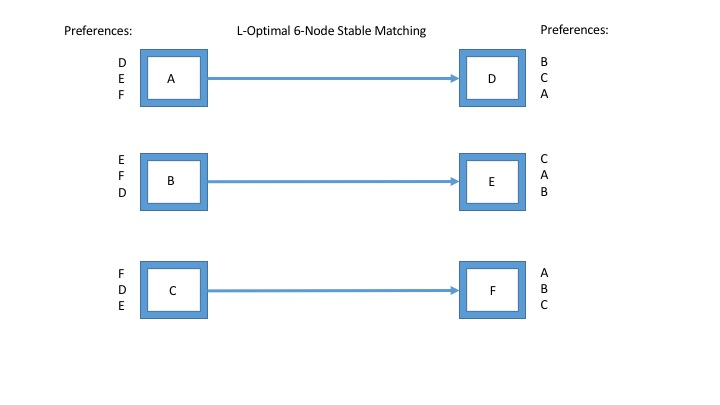
\includegraphics[scale=0.5]{lOptimal}\\
\indent Same example showing R-optimal is worst for L:\\
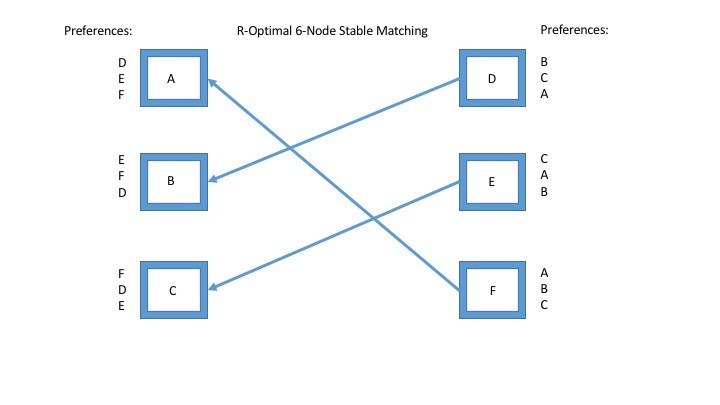
\includegraphics[scale=0.5]{rOptimal}\\\\
\indent To generalize this arrangement to 2n nodes, arrange the nodes in numerical order, nodes i = 1 to n in column L, and nodes j = n+1 to 2n, in column R.  For all nodes in L, most favored pairing is to node $i+n$, and least favored pairing is to node $i+n-1$, except for node 1, whose least favorite pairing is to node $2n$.  For all nodes in R, most favored pairing is to node (j-n+1), except for node 2n, who prefers node 1 to all other nodes.  Column R nodes' least favorite pairing is to node(j-n).\\
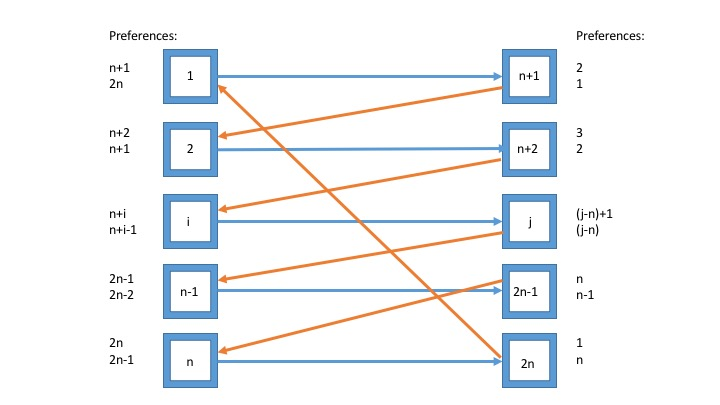
\includegraphics[scale=0.5]{2n}
\end{document}  